\documentclass[conference,flushend]{iaria} % (based on IEEEtran.cls)
% The class iaria.cls loads biblatex/biber with correct IARIA settings
% as well as a set of common packages (times, inputenc[utf8], fontenc[T1],
% graphicx, xcolor, url, orcidlink, hyperref, extdash[shortcuts])
\addbibresource{references.bib}
\title{Minimal Working Example of an IARIA Paper}
\author{
  \IEEEauthorblockN{%
    Jakob Löw\orcidlink{0009-0006-7088-8684}, Kevin Mayer\orcidlink{0000-0002-5597-3913}, Hans-Joachim Hof\orcidlink{0000-0002-6930-9271}}
  \IEEEauthorblockA{%
    CARISSMA Institute of Electric, Connected and Secure Mobility \\
    University of applied sciences Ingolstadt \\
    Ingolstadt, Germany \\
    e-mail: {\tt$\lbrace$jakob.loew\,|\,kevin.mayer\,|\,hof$\rbrace$@thi.de}
} }
\begin{document}
\maketitle
\begin{abstract}
This paper is a minimal working example.
% TODO: copy some parts from expose introduction?
\end{abstract}
\begin{IEEEkeywords}
minimal; MWE; IARIA.
\end{IEEEkeywords}

\section{Introduction}
Many countries are currently transitioning away from combustion engine vehicles towards battery electric ones.
This transition is happening at a rapid rate, because buying an electric vehicle often gets incentivised through tax reductions or straight refunds \cite{stats_electricvehicles}.
With people buying more and more electric vehicles, the demand for charging infrastructure rises.
In Germany not only electric vehicles, but also the buildup of charging infrastructure got heaviliy subsidized by the government.
This high demand and government incentives resulted in a rapid growth in charging station numbers, suppliers and operators \cite{stats_chargepoints}.
Due to the rushed development, the cybersecurity of current charging stations is below average compared to other cyberphysical systems \cite{nasr_power_2022, johnson_review_2022, ahalawat_security_2022}.
Recently cybersecurity researchers investigating charging backend infrastructure have found a range of text book vulernabilities, such as SQL injection, cross site scripting or unauthenticated remote update procedures \cite{nasr_power_2022}. %
%% \cite{gonium_talk} - gonium talk about charging stations: TODO often other vulnerabilities
%% \cite{garofalaki_electric_2022} - OCPP security issues and challenges
\\
In order to charge vehicle batteries fast charging stations perform high level communication with the vehicle, exchanging charging conditions and limits. The ISO15118 standard was created to allow interoperability between charging stations and vehicles of different manufacturers.
While this paper will briefly cover communication aspects of basic charging stations, its focus is on high level communication between DC fast charging stations and the ISO15118 standard.
% TODO extend this as transition to ISO15118 / high level charging

\section{Charging Station Communication}
Electricity generally comes in two forms: alternating current (AC) and direct current (DC).
While power grids are usually AC, batteries need to be charged using DC.
Therefore the AC needs to be converted to DC either in the car or in the charging station itself.
While cars usually come with an onboard AC to DC converter for charging the onboard battery their power is usually limited between 7 and 22 kW.
In order to achieve higher charging powers, a fast charging station provides a stationary AC to DC converter. Placing it outside of the car removes weight requirements, simplifies cooling and thus allows higher charging currents. \\
In general charging stations can be divided into three categories:
\begin{enumerate}
\item Unmetered AC charging (often used in residential buildings)
\item Commercial AC charging stations
\item DC fast charging stations
\end{enumerate}%
%
The following subsections describe the communication and payment mechanisms of these three kinds of charging stations as well as the included security concepts.

\subsection{Low Level Communication}
AC charging stations usually supply grid power directly, making them just sockets with some very basic communication to the vehicle.

% refs:
%% \cite{antoun_detailed_2020} - claims grid communication exists, claims home chargers have high-level communication with vehicles
%% \cite{IEC61851} - resistor & PWM communication

\subsection{High Level Communication}
DC charging stations on the other hand are required to communicate to the vehicle for properly supplying the correct voltage and power to the battery.
For this high level communication the industry standard ISO15118 was created, enabling interoperability between different vehicle manufacturers and charging station vendors.
While this standard allows possibilities for payment processing and value added services, it also comes with a lot of security implications.
% TODO extend this
\subsection{ISO15118 Security Concepts}
% TODO: PnC, TLS, TLS-downgrade
\subsection{Other Communication Standards}
% chademo, GB/T, MCS, ...

\section{Charging station technologies and vendors}
%% \cite{das_electric_2020} - EV market share, charging standards list
%% TODO: add vendor market analysis
%% TODO: add charge port analysis
\begin{figure}[ht]
    \centering
    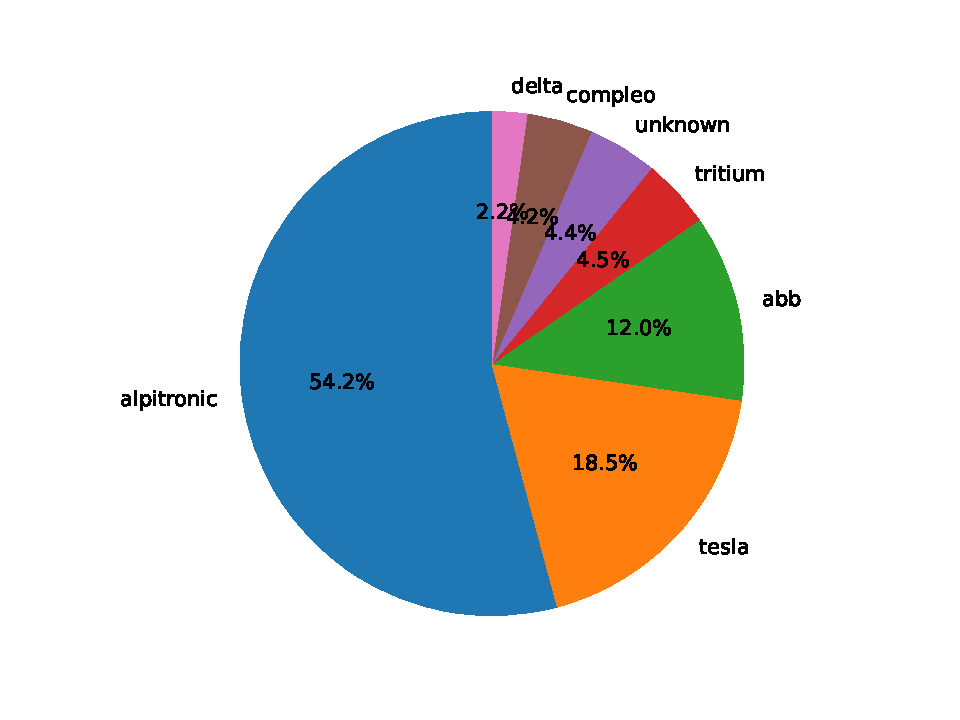
\includegraphics[width=.489\textwidth]{graphs/market_analysis.pdf}
    \caption{CCS charging station vendor market share}
    \label{fig:marketshare}
\end{figure}

\begin{figure}[ht]
    \centering
    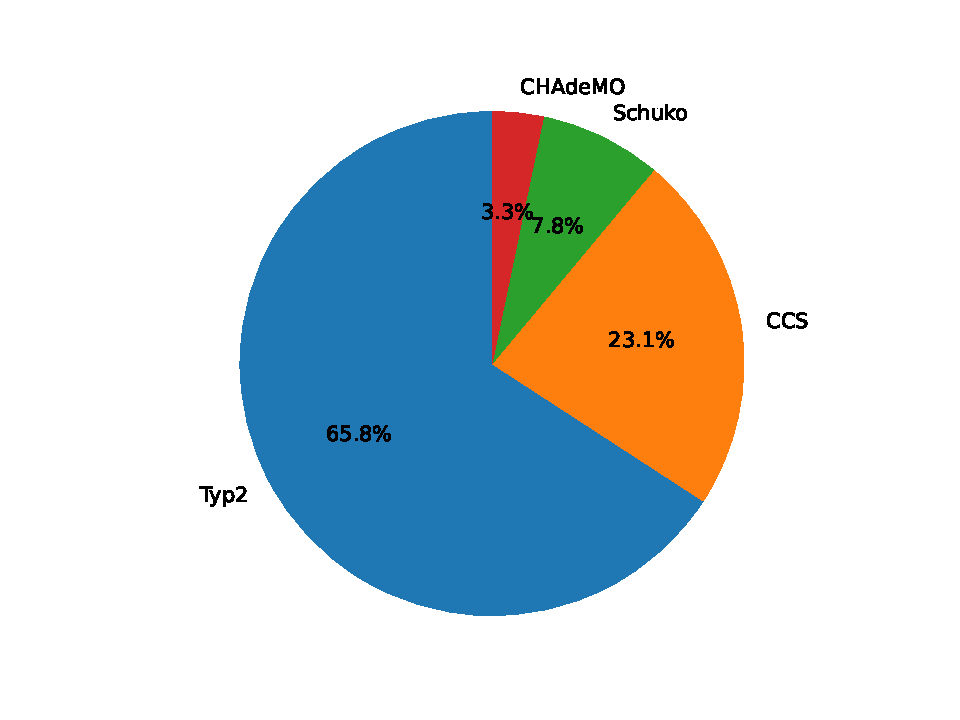
\includegraphics[width=.489\textwidth]{graphs/socket_analysis.pdf}
    \caption{Charging station socket market share}
    \label{fig:sockets}
\end{figure}

\begin{figure}[ht]
    \centering
    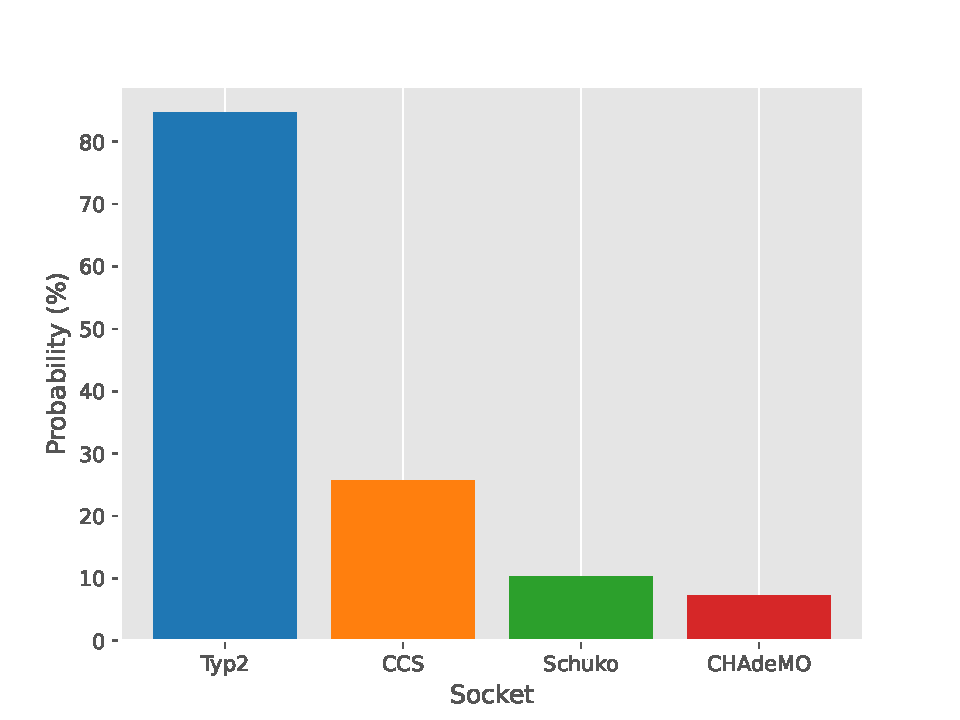
\includegraphics[width=.489\textwidth]{graphs/socket_probability.pdf}
    \caption{Probability to find socket X at a random charging location}
    \label{fig:socketsprob}
\end{figure}



\section{Charging Station Architectures}
% TODO: explain proposed architectures
%% \cite{acharya_cybersecurity_2020} - very good architecture schematic of grid/charging station/EV connections and communication.

\subsection{Proposed architectures}
%% \cite{deb_review_2021} - DC bus architektur
\subsection{Integration of battery storage and photovoltaics}
% TODO
\subsection{Independent charging stations}
% TODO: alpitronic
\subsection{DC Bus Systems}
% TODO: Tesla v4

\section{Attack Vectors and Impact}
%% \cite{bao_threat_2018} - ISO15118 threat analysis
%% \cite{kohler_brokenwire_2023} - jamming powerline in ISO15118 communication
%% \cite{nasr_chargeprint_2023} - framework for backend service security analysis

% impact:
%% \cite{sanghvi_cybersecurity_2021} - energy simulation using OpenDSS - impact of vulnerabilities
%% \cite{acharya_cybersecurity_2020} - very good architecture schematic of grid/charging station/EV connections and communication.

% TODO: subsections

\section{Cybersecurity State}
%% \cite{sklyar_chargepoint_nodate} - pentest of chargepoint charging station: many text-book vulnerabilities / buffer overflows / linux fails (suid bit, ssh rev tunnel to mothership, ...)

\section{Conclusion}
%% \cite{mccarthy_cybersecurity_2023} - NIST guidelines for IT security measures in EVs / charging stations / ... - as a recommendation?

\printbibliography
\end{document}
